\section{Cenário de Teste 1}

Este cenário está dividido em 5 (cinco) exemplos, os quais são apresentados a seguir, contemplando todo o processo de auto-localização
em cada exemplo, a partir da apresentação das imagens a seguir, Figura \ref{img:cen1_ex1} a Figura \ref{img:real_cen1_ex5}.

\subsection{Exemplo 1}

Exemplo utilizando 200 partículas:

{\centering
\includegraphics[scale=0.4]{figuras/cen1_ex1.eps}
\captionof{figure}{Cenário 1 - Exemplo 1.}
\label{img:cen1_ex1}
\par}

{\centering
\includegraphics[scale=0.2]{figuras/real_cen1_ex1.eps}
\captionof{figure}{Posição Real do Cenário 1 - Exemplo 1.}
\label{img:real_cen1_ex1}
\par}

\subsection{Exemplo 2}

Exemplo utilizando 400 partículas:

{\centering
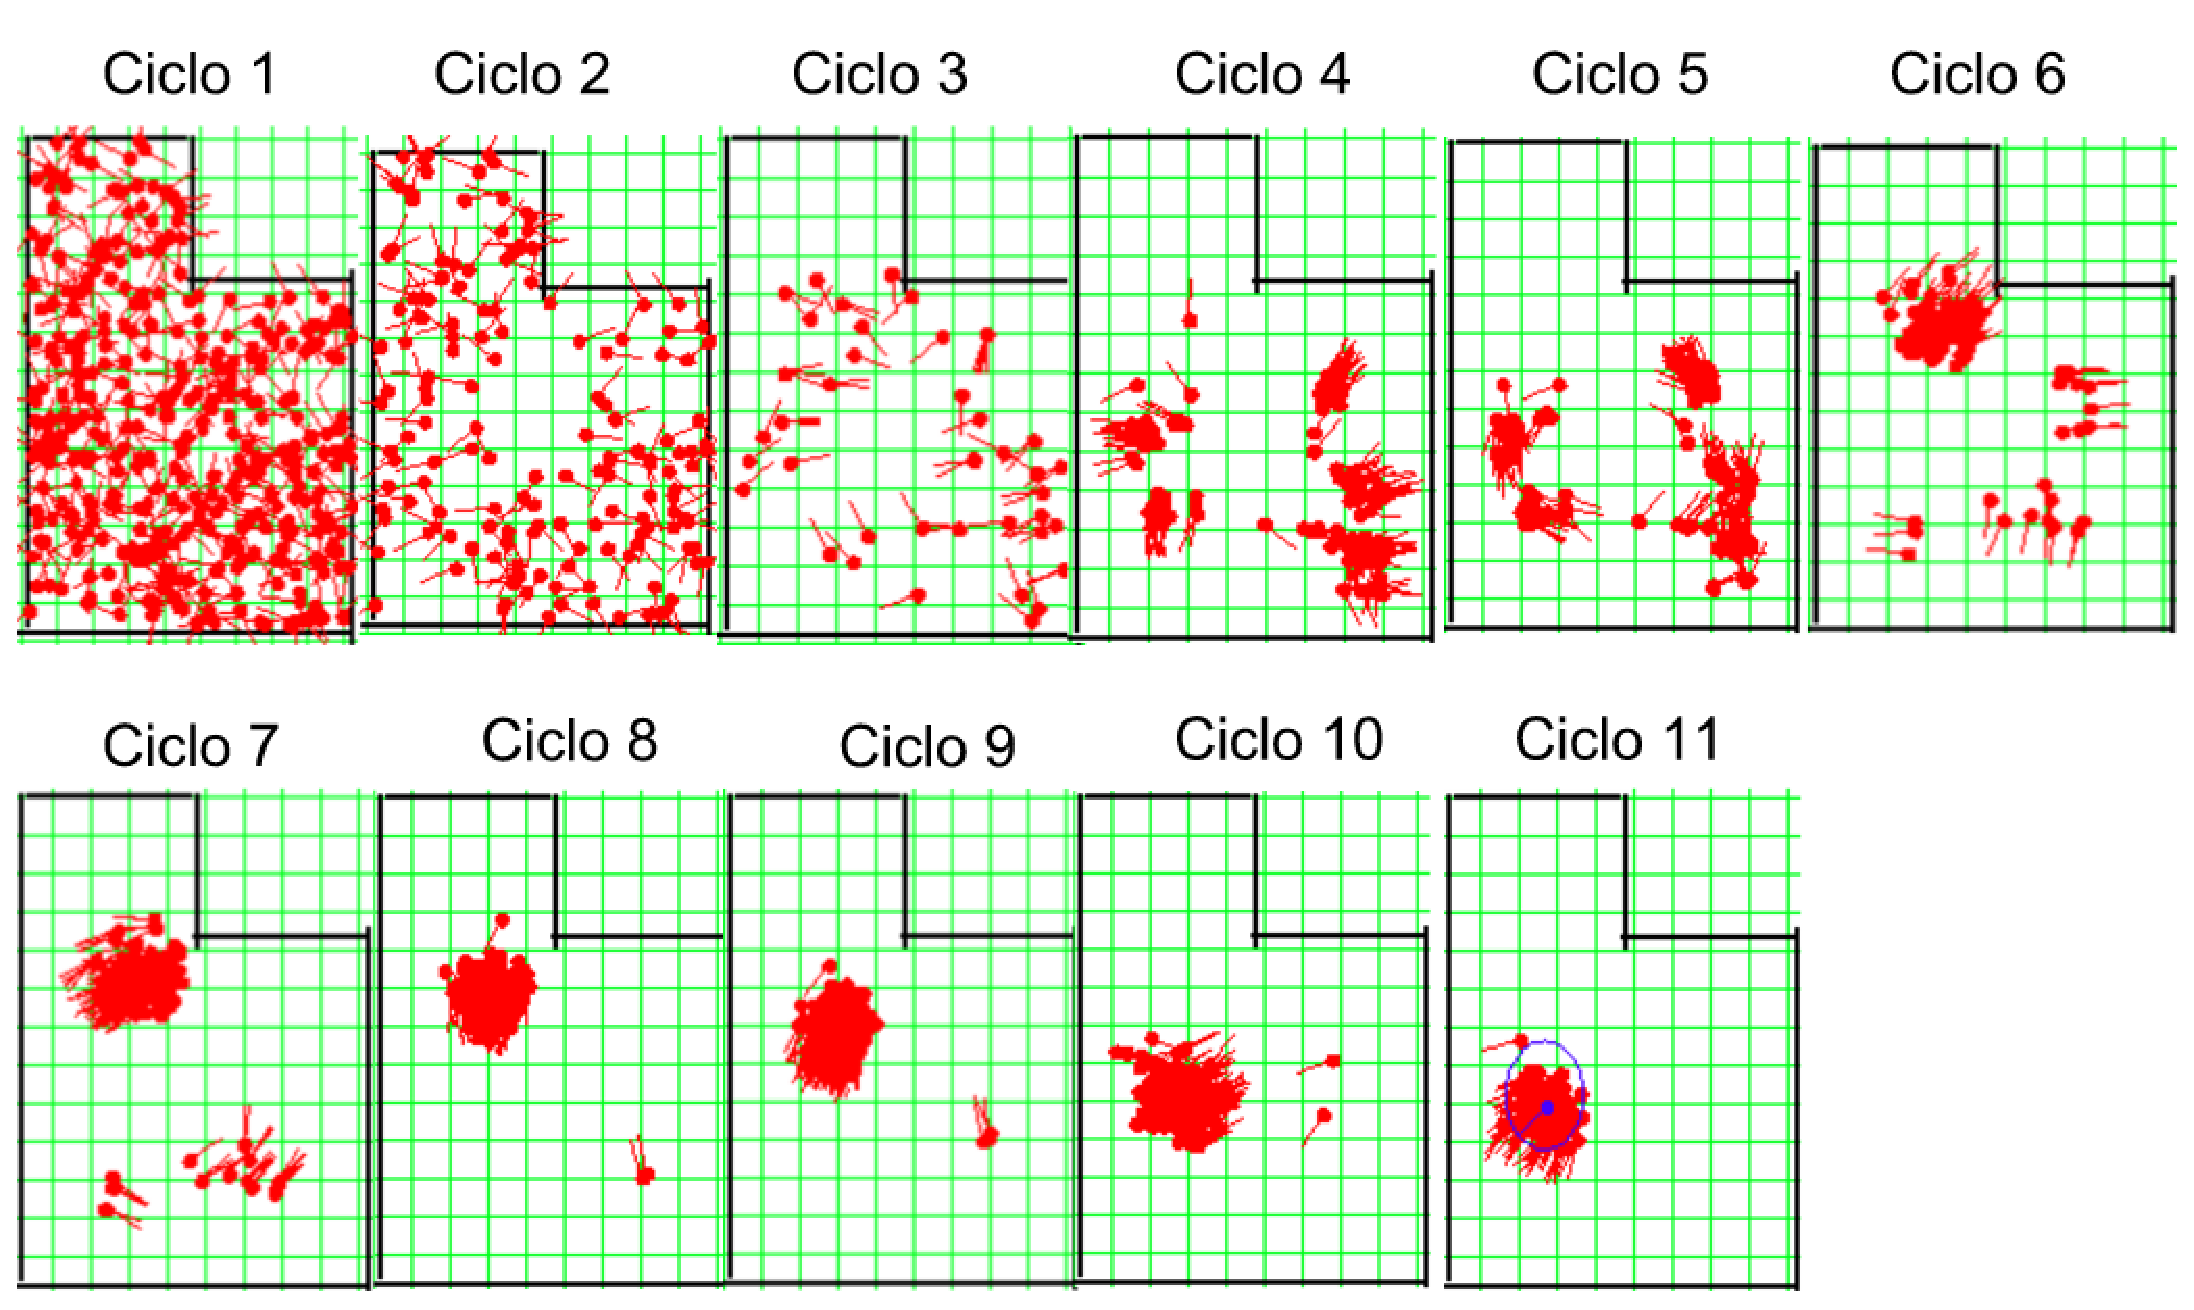
\includegraphics[scale=0.4]{figuras/cen1_ex2.eps}
\captionof{figure}{Cenário 1 - Exemplo 2.}
\label{img:cen1_ex2}
\par}

{\centering
\includegraphics[scale=0.2]{figuras/real_cen1_ex2.eps}
\captionof{figure}{Posição Real do Cenário 1 - Exemplo 2.}
\label{img:real_cen1_ex2}
\par}

\subsection{Exemplo 3}

Exemplo utilizando 500 partículas:

{\centering
\includegraphics[scale=0.4]{figuras/cen1_ex3_1.eps}
\captionof{figure}{Cenário 1 - Exemplo 3 Parte 1.}
\label{img:cen1_ex3_1}
\par}

{\centering
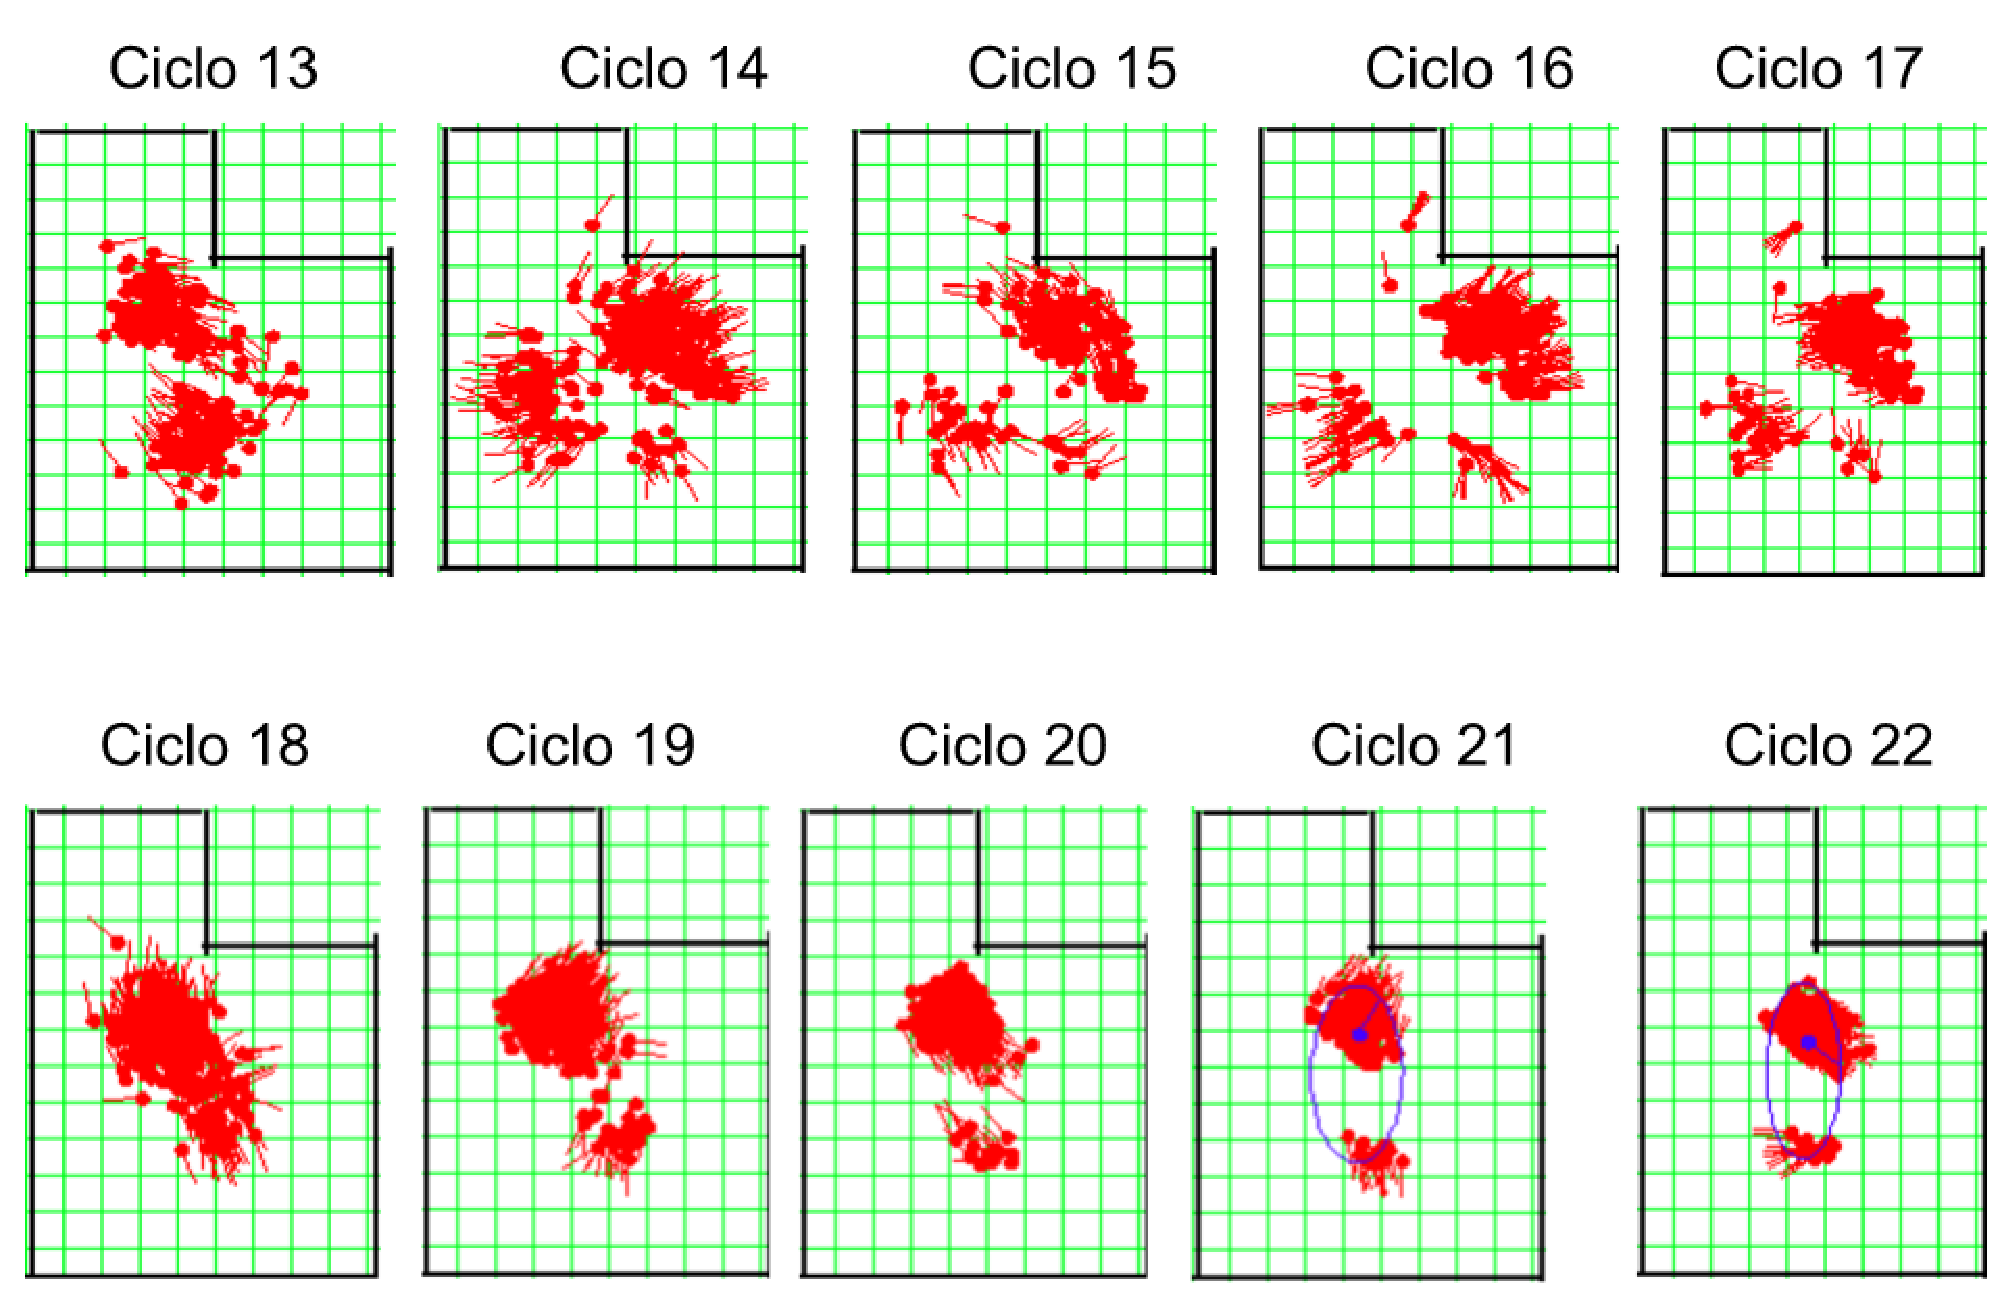
\includegraphics[scale=0.4]{figuras/cen1_ex3_2.eps}
\captionof{figure}{Cenário 1 - Exemplo 3 Parte 2.}
\label{img:cen1_ex3_2}
\par}

{\centering
\includegraphics[scale=0.2]{figuras/real_cen1_ex3.eps}
\captionof{figure}{Posição Real do Cenário 1 - Exemplo 3.}
\label{img:real_cen1_ex3}
\par}

\subsection{Exemplo 4}

Exemplo utilizando 100 partículas:

{\centering
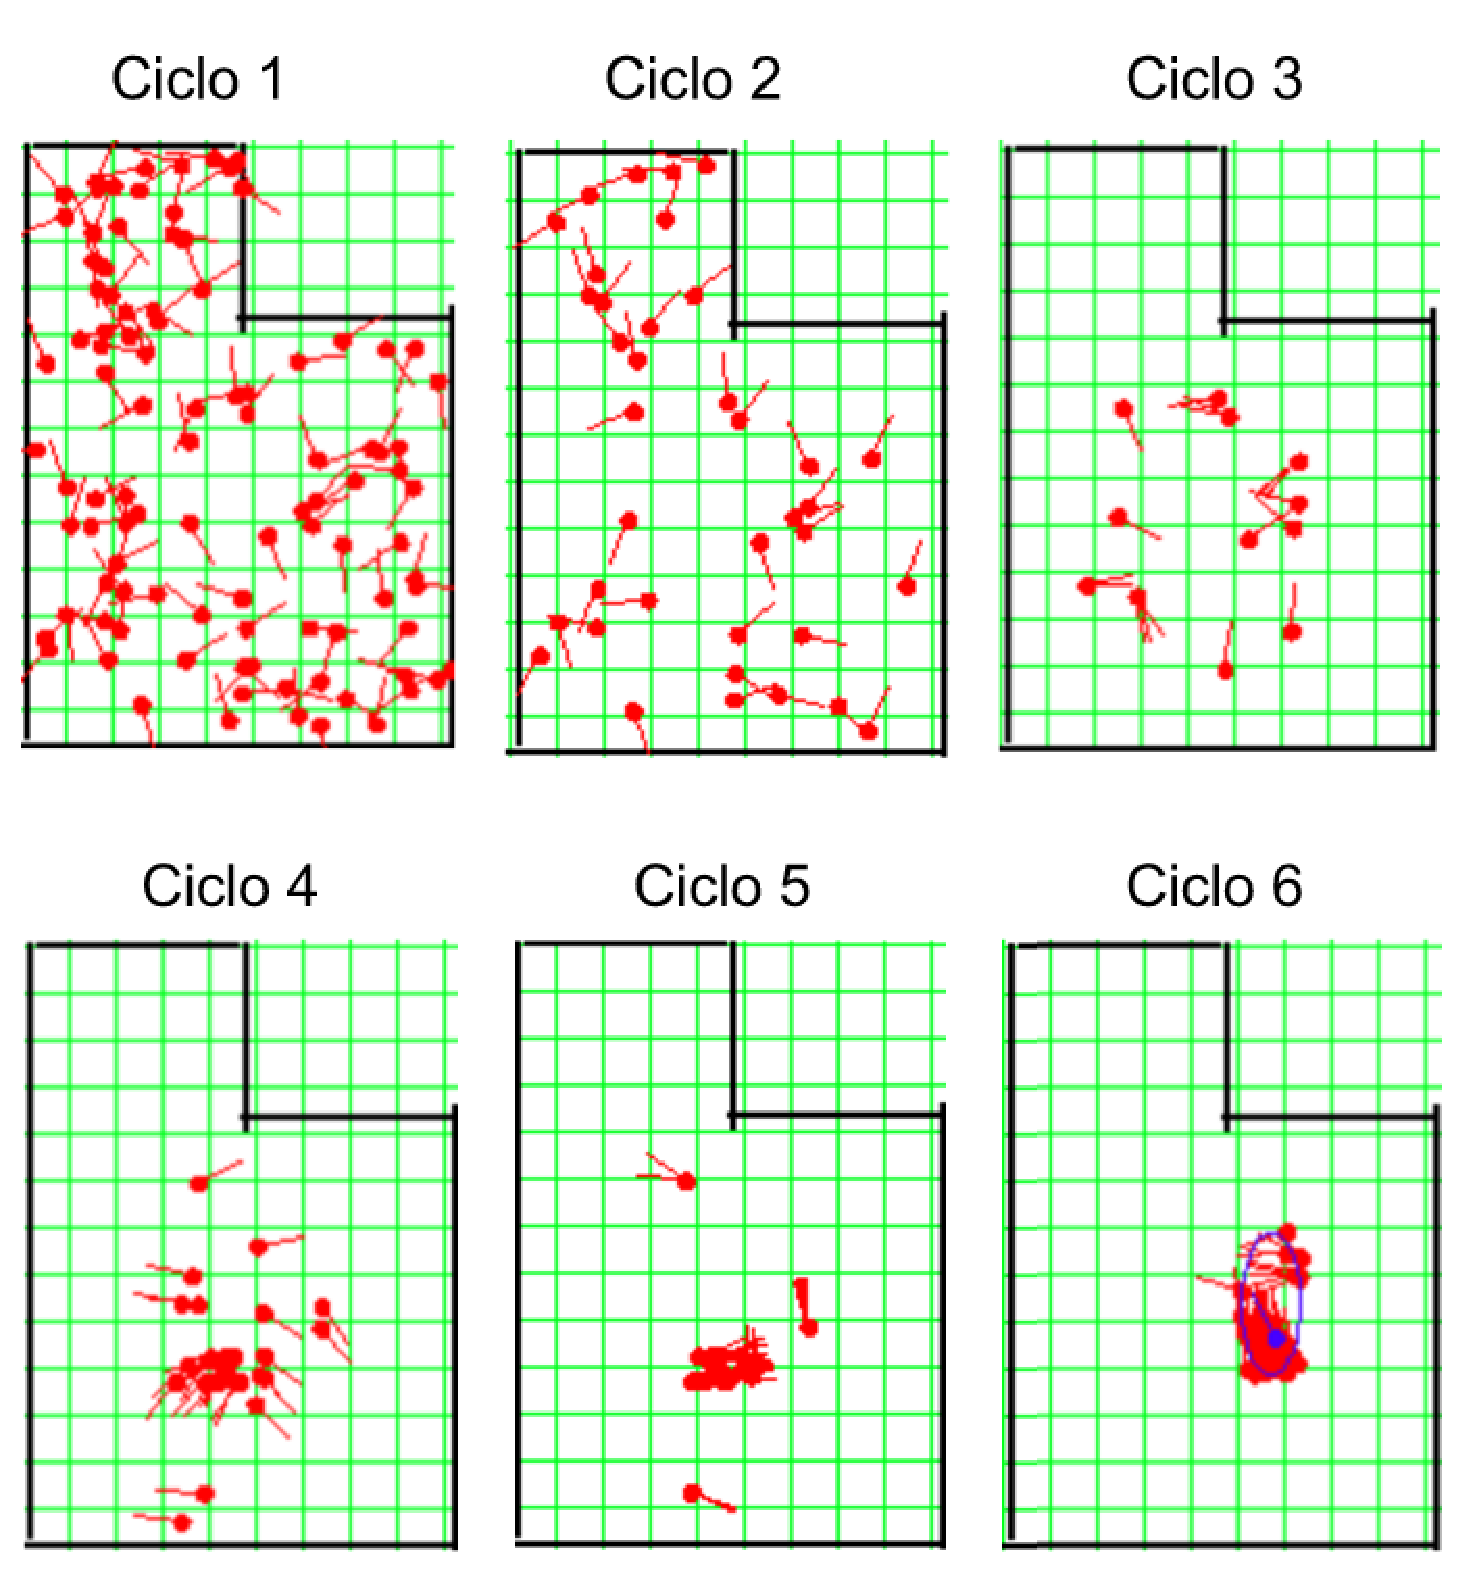
\includegraphics[scale=0.4]{figuras/cen1_ex4.eps}
\captionof{figure}{Cenário 1 - Exemplo 4.}
\label{img:cen1_ex4}
\par}

{\centering
\includegraphics[scale=0.2]{figuras/real_cen1_ex4.eps}
\captionof{figure}{Posição Real do Cenário 1 - Exemplo 4.}
\label{img:real_cen1_ex4}
\par}

\subsection{Exemplo 5}

Exemplo utilizando 150 partículas:

{\centering
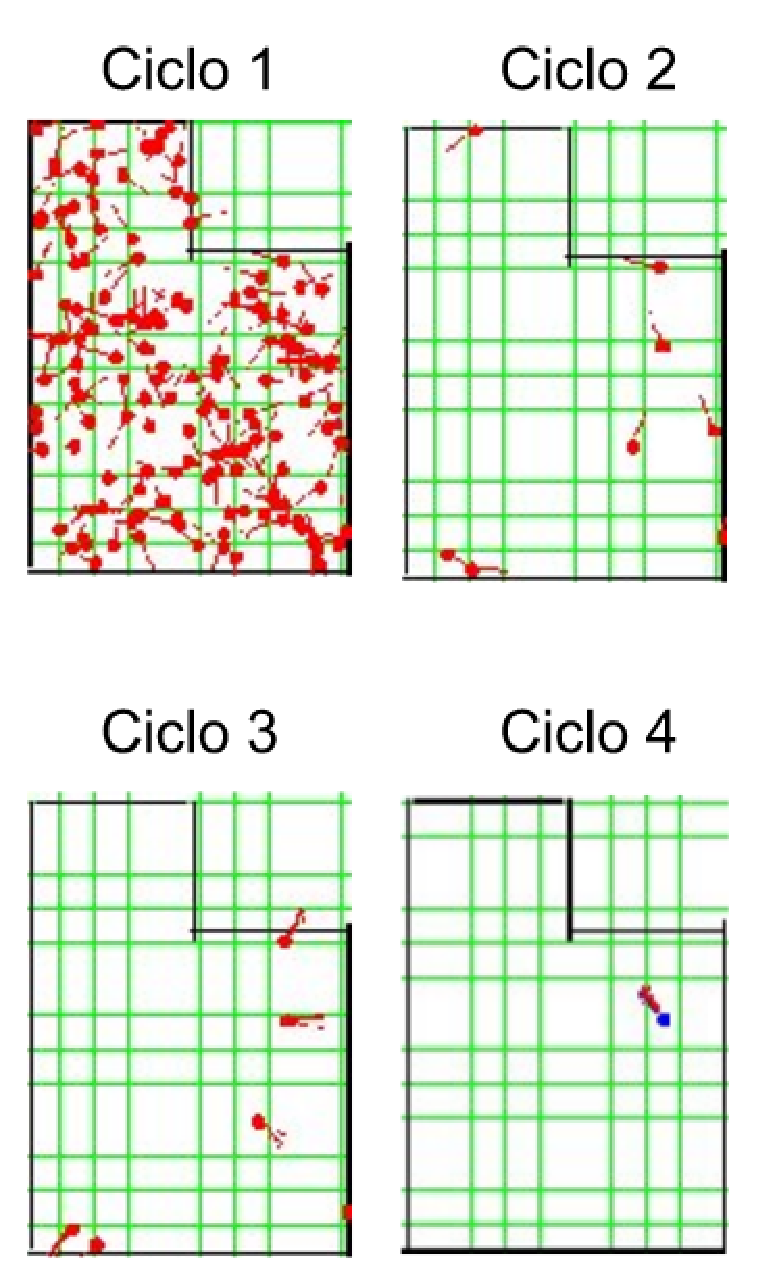
\includegraphics[scale=0.4]{figuras/cen1_ex5.eps}
\captionof{figure}{Cenário 1 - Exemplo 5}
\label{img:cen1_ex5}
\par}

{\centering
\includegraphics[scale=0.2]{figuras/real_cen1_ex5.eps}
\captionof{figure}{Posição Real do Cenário 1 - Exemplo 5.}
\label{img:real_cen1_ex5}
\par}
